% This must be in the first 5 lines to tell arXiv to use pdfLaTeX, which is strongly recommended.
\pdfoutput=1
% In particular, the hyperref package requires pdfLaTeX in order to break URLs across lines.


\documentclass[11pt]{article}


% Change "review" to "final" to generate the final (sometimes called camera-ready) version.
% Change to "preprint" to generate a non-anonymous version with page numbers.
\usepackage{acl}

% Standard package includes
\usepackage{times}
\usepackage{latexsym}
\usepackage{rotating}
\usepackage{natbib}
\usepackage{varioref}  
\usepackage{graphicx}


% For proper rendering and hyphenation of words containing Latin characters (including in bib files)
\usepackage[T1]{fontenc}
% For Vietnamese characters
% \usepackage[T5]{fontenc}
% See https://www.latex-project.org/help/documentation/encguide.pdf for other character sets

% This assumes your files are encoded as UTF8
\usepackage[utf8]{inputenc}

% This is not strictly necessary, and may be commented out,
% but it will improve the layout of the manuscript,
% and will typically save some space.
\usepackage{microtype}

% This is also not strictly necessary, and may be commented out.
% However, it will improve the aesthetics of text in
% the typewriter font.
\usepackage{inconsolata}

%Including images in your LaTeX document requires adding
%additional package(s)
\usepackage{graphicx}
\usepackage{setspace}
\usepackage{graphicx}
\usepackage{listings}
\usepackage{xcolor}
\usepackage{subcaption}
\usepackage{import}

\usepackage{cleveref}

% Custom command for appendix figures
\newcommand{\appfigure}[1]{Figure~\ref{#1}}


% Add this line to define \textrussian command
\newcommand{\textrussian}[1]{\foreignlanguage{russian}{#1}}

\lstset{
    language=Python,
    breaklines=true,
    basicstyle=\small\ttfamily,  % Reduced font size
    keywordstyle=\color{blue}\bfseries,  % Bold blue keywords
    stringstyle=\color{green!50!black},  % Dark green strings
    commentstyle=\color{gray}\itshape,  % Italic gray comments
    numbers=left,  % Add line numbers on the left
    linewidth=0.5\textwidth,  % Increased width to 95% of text width
    showspaces=false,
    showstringspaces=false,  % Don't show spaces in strings
    captionpos=b,  % Place caption at the bottom
    tabsize=4,  % Set tab size to 4 spaces
    keepspaces=true,  % Keep spaces in code
    xleftmargin=\parindent,  % Align with paragraph indentation
}
\usepackage{graphicx}
\graphicspath{{../plots/}}



\begin{document}

\nolinenumbers  % Add this line to ensure line numbers are turned off


\title{NLP Course Report}
\author{Hans Peter Lyngsøe, pvr448}

\maketitle

\section{Week 1}
% (a) Explore the dataset from https://huggingface.co/datasets/coastalcph/tydi_xor_rc. 
% Familiarize yourself with the dataset card, download the dataset and explore its columns. 
% Summarize basic data statistics for training and validation data in each of the languages 
% Fi, Ja and Ru.
\begin{enumerate}
    \item[(a)] 

    Basic statistics:
    \begin{itemize}
        \item the data is quite evenly distributed across the 3 languages.
        \item We note that there are more answerable than unanswerable by a factor of 10-1.Which means we accuracy becomes a meaningless measure for performance.
        \item train\_set: 15326
        \item val\_set: 3028
    \end{itemize}

    \begin{figure}[ht]
        \centering
        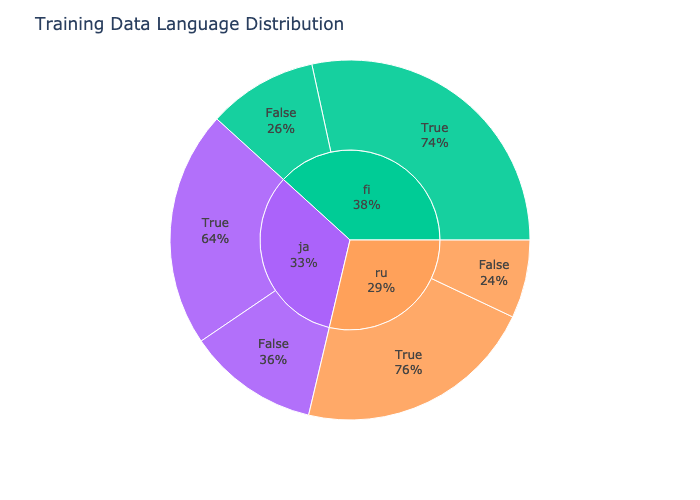
\includegraphics[width=0.3\textwidth]{week1_a_dataset.png}
        \caption{Distribution of labels in the dataset}
        \label{fig:label_distribution}
    \end{figure}

    \begin{figure}[ht]
        \centering
        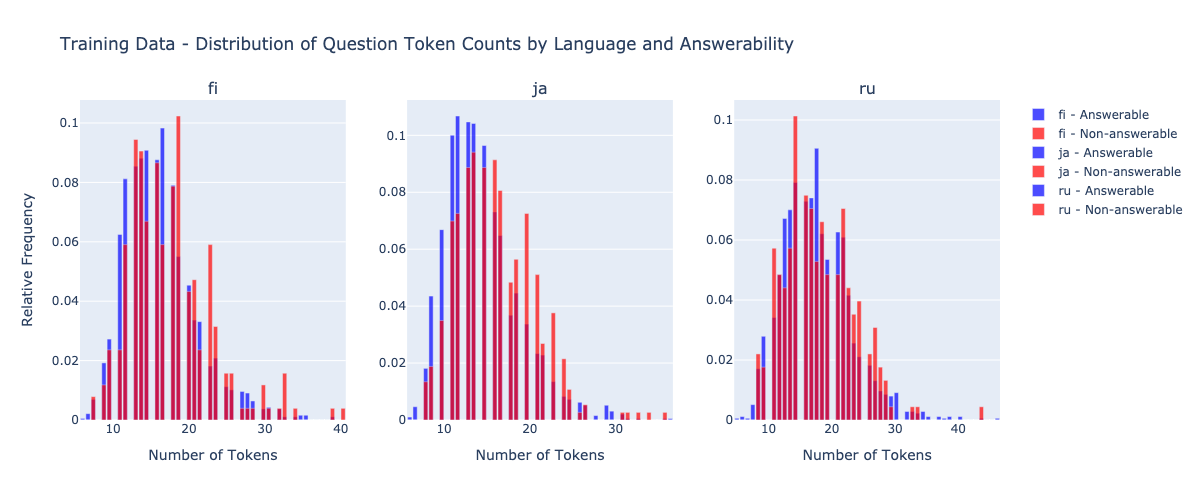
\includegraphics[width=0.5\textwidth]{week1_a_lang_token_distribution_normalized.png}
        \caption{normalized Histogram for token count(using llama3 tokenizer) of answerable/unanswerable questions in the dataset}
        \label{fig:language_distribution}
    \end{figure}

    % (b) For each of the languages Finnish, Japanese and Russian, report the 5 most common 
    % words in the questions from the training set. What kind of words are they?
    \item[(b)] 

    In order to get a faithful representation of the most meaningful words, we opt to filter out stopwords arguing that these words are not meaningful and does not carry information about the question.
    We use the NLP library, spacy, that provides an index of stopwords for each language. Additionally we remove common symbols like '.' and '?' and other common tokens that were not part of the stopwords

    We use the fact that both finnish and russian use spaces to seperate their words, and thus we can extract distinct words using the space as delimiter.
    Japanese is somewhat different as a language, and it is unclear whether naive splitting on spaces is meaningful. Thus we use a japanese specific tokenizer to parse sentences into words.
    we get the following results:

    \begin{figure}[t]
        \centering
        \begin{subfigure}[b]{0.1\textwidth}
            \centering
            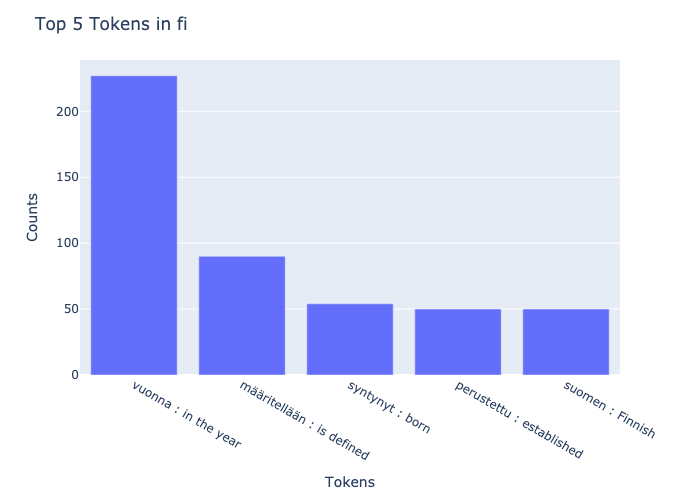
\includegraphics[width=\textwidth]{week1_b_top_5_tokens_fi.png}
            \caption{Finnish}
            \label{fig:top_5_tokens_fi}
        \end{subfigure}
        \hfill
        \begin{subfigure}[b]{0.1\textwidth}
            \centering
            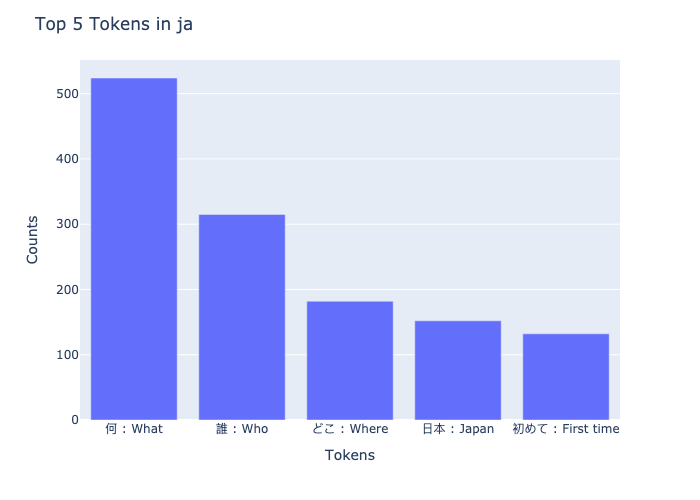
\includegraphics[width=\textwidth]{week1_b_top_5_tokens_ja.png}
            \caption{Japanese}
            \label{fig:top_5_tokens_ja}
        \end{subfigure}
        \hfill
        \begin{subfigure}[b]{0.1\textwidth}
            \centering
            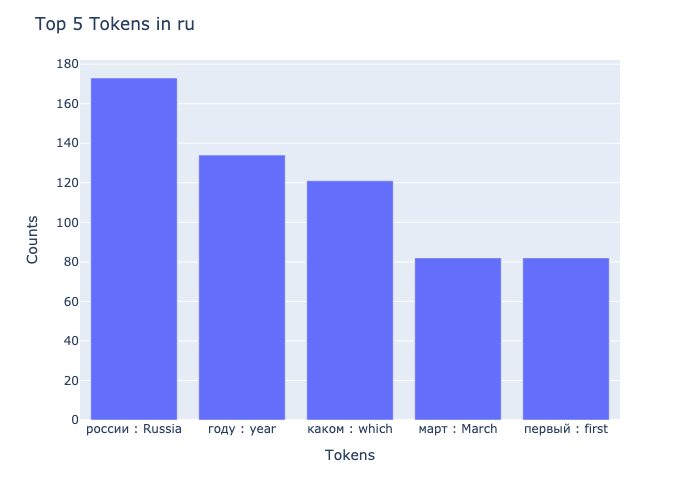
\includegraphics[width=\textwidth]{week1_b_top_5_tokens_ru.png}
            \caption{Russian}
            \label{fig:top_5_tokens_ru}
        \end{subfigure}
        \caption{Top 5 tokens in Finnish, Japanese, and Russian}
        \label{fig:top_5_tokens_all}
    \end{figure}

    in all 3 cases words like 'year'/'year of' are in the top 5. likewise the names of the respective capital cities of the countries are in the top 5 in all 3 cases.
    Other words like 'first'. In general words that help describe facts and words that are preprosition words are common.

    %%NOTE: todo use an embedding model to get a sense for the meaning of the words, consider how you do tokenization and 

    % (c) Implement a rule-based classifier that predicts whether a question is answerable 
    % or impossible, only using the document (context) and question. You may use machine 
    % translation as a component. Use the answerable field to evaluate it on the validation set. 
    % What is the performance of your classifier for each of the languages Finnish, Japanese and Russian?
    \item[(c)] 
    
    % TODO use 


    We expect that as a rough heuristic that longer questions are harder to answer. 
    We make a scatter plot for each language with the word length of the question against the answerability of the question.
    We see a slight correlation between question length and answerability(can be found Figure~\ref{fig:scatter_week1_c_fi}, \ref{fig:scatter_week1_c_ja}, and \ref{fig:scatter_week1_c_ru} ). 
    Based on this information, we decide to make a rule-based classifier that predicts unanswerable for questions above a language-specific threshold determined based on the scatter plot.

    we get the following results on the validation set:

    %% ja: {'accuracy': 0.5877192982456141, 'balanced_accuracy': 0.53745129167268, 'f1': 0.6907894736842105, 'precision': 0.6542056074766355, 'recall': 0.7317073170731707}
    %% ru: {'accuracy': 0.7121212121212122, 'balanced_accuracy': 0.4964788732394366, 'f1': 0.831858407079646, 'precision': 0.7157360406091371, 'recall': 0.9929577464788732}
    %% fi: {'accuracy': 0.6912878787878788, 'balanced_accuracy': 0.5132645803698435, 'f1': 0.81068524970964, 'precision': 0.7255717255717256, 'recall': 0.9184210526315789}
    %% all: {'accuracy': 0.6630434782608695, 'balanced_accuracy': 0.5284132271513975, 'f1': 0.783418723800652, 'precision': 0.7031772575250836, 'recall': 0.8843322818086226}
    \begin{table}[ht]
        \centering
        \resizebox{0.9\columnwidth}{!}{
        \begin{tabular}{|l|c|c|c|c|}
            \hline
            Language & Balanced Accuracy & F1 Score & Precision & Recall \\
            \hline
            All & 0.5284 & 0.7834 & 0.7032 & 0.8843 \\
            Fi & 0.5133 & 0.8107 & 0.7256 & 0.9184 \\
            Ja & 0.5375 & 0.6908 & 0.6542 & 0.7317 \\
            Ru & 0.4965 & 0.8319 & 0.7157 & 0.9930 \\
            \hline
        \end{tabular}
        }
        \caption{Performance metrics of the rule-based classifier on the validation set}
        \label{tab:classifier_performance}
    \end{table}

    Performance is poor, and there are many downsides to this approach: 
    first of all, although length might be somewhat correlated with answerability this is a vary noisy signal. 
    The as length is a bad measure of complexity.
    Furthermore we are putting a lot of faith in the tokenization step. And the predictions of our model could be meaningfully change with a different tokenization scheme.
    We also note that this is barely better than sampling from a bernoulli distribution with the mean of the answerability in the training data.

\end{enumerate}

\section{Week 37 (9--15 September)}
% Let k be the number of members in your group (k ∈ {1, 2, 3}). Implement k different 
% language models for the questions in the three languages Finnish, Japanese and Russian, 
% as well as for the document contexts in English (total k × 4 language models), using the 
% training data. Evaluate each of them on the validation data, report their performance 
% and discuss the results.

We train 3 different N-Gram models, one for each language.

Curiously enough we find that as we scale the number of tokens in the training data, the performance of the model gets worse.
\begin{table}[ht]
    \centering
    \resizebox{0.9\columnwidth}{!}{%
    \begin{tabular}{|l|r|r|}
        \hline
        Language & Training Tokens/Words & Perplexity \\
        \hline
        Ja & 24,533 & 548.79 \\
        Ru & 16,526 & 140.53 \\
        Fi & 13,013 & 91.90 \\
        Context (English) & 751,154 & 616.85 \\
        \hline
    \end{tabular}
    }
    \caption{Language Model Performance}
    \label{tab:language_model_performance}
\end{table}



\section{Week 38 (16--22 September)}
% Let k be the number of members in your group. For each of the three languages Finnish, 
% Japanese and Russian separately, using the training data, train k different classifiers 
% that receive the document (context) and question as input and predict whether the question 
% is answerable or impossible given the context. Evaluate the classifiers on the respective 
% validation sets, report and analyse the performance for each language and compare the 
% scores across languages.

We train a linear classifier on embeddings from OpenAI's 'text-embedding-ada-002' model. 
The input features are the concatenated embeddings of the question and context (3072 dimensions). 
We use binary cross-entropy loss for training.

\begin{table}[ht]
    \centering
    \resizebox{0.9\columnwidth}{!}{
    \begin{tabular}{|l|l|c|c|c|c|c|c|}
    \hline
    Training & Evaluation & Context & D\_in & Expansion & Balanced & Precision & Recall \\
    & & & & factor & Accuracy & & \\
    \hline
    Fi & Fi & No & 1536 & 2 & 0.9031 & 0.9825 & 0.9492 \\
    Fi & Fi & Yes & 3072 & 2 & 0.7562 & 0.9466 & 0.9767 \\
    Fi & Ja & No & 1536 & 2 & 0.8293 & 0.9460 & 0.8904 \\
    Fi & Ja & Yes & 3072 & 2 & 0.6366 & 0.8652 & 0.9439 \\
    Fi & Ru & No & 1536 & 2 & 0.9184 & 0.9943 & 0.9278 \\
    Fi & Ru & Yes & 3072 & 2 & 0.8556 & 0.9840 & 0.9840 \\
    Fi & All & Yes & 3072 & 2 & 0.5670 & 0.8981 & 0.9902 \\
    Fi & All & No & 1536 & 2 & 0.8810 & 0.9775 & 0.9246 \\
    Ja & Fi & No & 1536 & 2 & 0.8543 & 0.9716 & 0.9407 \\
    Ja & Fi & Yes & 3072 & 2 & 0.5247 & 0.8987 & 0.9958 \\
    Ja & Ja & No & 1536 & 2 & 0.7625 & 0.9105 & 0.9519 \\
    Ja & Ja & Yes & 3072 & 2 & 0.5244 & 0.8274 & 1.0000 \\
    Ja & Ru & No & 1536 & 2 & 0.9251 & 0.9919 & 0.9866 \\
    Ja & Ru & Yes & 3072 & 2 & 0.5896 & 0.9540 & 0.9973 \\
    Ja & All & Yes & 3072 & 2 & 0.5300 & 0.8903 & 0.9975 \\
    Ja & All & No & 1536 & 2 & 0.8162 & 0.9574 & 0.9574 \\
    Ru & Fi & No & 1536 & 2 & 0.6438 & 0.9231 & 0.9661 \\
    Ru & Fi & Yes & 3072 & 2 & 0.6789 & 0.9313 & 0.9470 \\
    Ru & Ja & No & 1536 & 2 & 0.7694 & 0.9143 & 0.9412 \\
    Ru & Ja & Yes & 3072 & 2 & 0.7585 & 0.9098 & 0.9439 \\
    Ru & Ru & No & 1536 & 2 & 0.7045 & 0.9664 & 1.0000 \\
    Ru & Ru & Yes & 3072 & 2 & 0.7955 & 0.9765 & 1.0000 \\
    Ru & All & No & 1536 & 2 & 0.7126 & 0.9314 & 0.9689 \\
    Ru & All & Yes & 3072 & 2 & 0.7436 & 0.9392 & 0.9623 \\
    \hline
    \end{tabular}%
    }
    \caption{Model performance for language-specific training and cross-language evaluation, with and without context}
    \label{tab:model_performance_cross_language}
\end{table}

from the results we see that the russian classifier achieves the highest balanced accuracy followed by the japanese and finnish.
this is unexpected as one would assume the quality of the embeddings would be higher for more common languages spoken online(ja > ru > fi).
Interestingly enough this trend is reversed if we exclusively train on the question embedding, disregarding the context. 
Where we observe a meaningful boost in performance for the finnish and japanese classifiers although we striclty have less information.

Additionally to better understand the difficulty of different languages we evaluate the classifier on the validation set of each language, including languages the model was not previously trained on.
Suprinsingly for the finnish and japanese classifiers perform better on the russian validation set than the validation set they themselves were trained on.
To get a better understanding of the impact. 


We also experiment with training a single model on all three languages, to better understand the value of multilingual data.

\begin{table}[ht]
    \centering
    \resizebox{0.9\columnwidth}{!}{
    \begin{tabular}{|l|l|c|c|c|c|c|c|}
    \hline
    Training & Evaluation & Context & D\_in & Expansion & Balanced & Precision & Recall \\
    & & & & Factor & Accuracy & & \\
    \hline
    All & Fi & No & 1536 & 2 & 0.9414 & 0.9933 & 0.9364 \\
    All & Fi & Yes & 3072 & 2 & 0.9225 & 0.9888 & 0.9343 \\
    All & Ja & No & 1536 & 2 & 0.6688 & 0.8741 & 0.9840 \\
    All & Ja & Yes & 3072 & 2 & 0.8663 & 0.9559 & 0.9278 \\
    All & Ru & No & 1536 & 2 & 0.7955 & 0.9765 & 1.0000 \\
    All & Ru & Yes & 3072 & 2 & 0.8810 & 0.9867 & 0.9893 \\
    \hline
    \end{tabular}%
    }
    \caption{Model performance for language-specific and combined training, with and without context}
    \label{tab:model_performance}
\end{table}


\section{Week 39 (23--29 September)}
% We now move from binary classification to span-based QA, i.e. identifying the
% span in the document that answers the question.
% Let k be the number of members in your group. Using the training data in
% Finnish, Japanese and Russian separately, train k different sequence labellers,
% which predict the tokens in a document context that constitute the answer to
% the corresponding question.9 You can decide whether to train one model per
% language or a single model for all three languages. Evaluate using a sequence la-
% belling metric on the validation set, report and analyse the performance for each
% language and compare the scores across languages. Note that if the question is
% unanswerable, a correct output must be empty (contain no tokens).

We experiment with various sequence labeling encoder-decoder models. 

We explore the finetuning of the following models:
distillbert as a baseline and deberta\_V3 as it is a state of the art model. Deberta performs the best.
However we note that there is a meaningful discrepancy between how the model performs on finnish vs russian and japanese. 
This is expected as distilbert and deberta are not explicitly trained on the respective languages.
Thus we also examine using the mt5 base model that is a t5 encoder decoder model, that is trained on all 3 target languages(https://huggingface.co/google/mt5-base).
Instead of doing a whole finetune we freeze the weights and use a lora adapter \cite{hu2021loralowrankadaptationlarge}. 
We use the same metrics, exact match and f1 score as established in the SQuAD v1 paper \cite{rajpurkar-etal-2018-know}.


\begin{table}[ht]
    \centering
    \resizebox{0.9\columnwidth}{!}{
    \begin{tabular}{|l|l|c|c|}
        \hline
        epoch & Language & Exact & F1 Score \\
        & & match & \\
        \hline
        0 & Fi & 0.7576 & 5.2205 \\
        0 & Ja & 0.8772 & 4.7133 \\
        0 & Ru & 0.0 & 5.4960 \\
        \hline
        2 & Fi & 40.7197 & 45.4617 \\
        2 & Ja & 49.3421 & 42.6790 \\
        2 & Ru & 41.9192 & 48.0977 \\
        \hline
        4 & Fi & 42.8030 & 45.6286 \\
        4 & Ja & 51.5351 & 44.4455 \\
        4 & Ru & 41.1616 & 48.0781 \\
        \hline
        6 & Fi & 41.8561 & 46.1020 \\
        6 & Ja & 50.0000 & 44.3151 \\
        6 & Ru & 41.9192 & 47.9060 \\
        \hline
        8 & Fi & 41.8561 & 46.1203 \\
        8 & Ja & 49.1228 & 44.8132 \\
        8 & Ru & 42.1717 & 48.2566 \\
        \hline
    \end{tabular}
    }
    \caption{Evaluation metrics for different languages}
    \label{tab:evaluation_metrics}
\end{table}

we observe that although distillbert performs the best before finetuning(epoch 0) deberta ends up outperforming it after finetuning.

\section{Week 40 (30 September--6 October)}
\label{sec:week40}
% Use the subset of the questions in Finnish, Japanese and Russian to train (or fine-tune) 
% an encoder-decoder model that receives the question and context as input and generates 
% the in-language answer. You can decide whether to train one model per language or a 
% single model for all three languages.

For this task we opt for finetuning a general pretrained multimodal large multilingural language model, Llama3-1-8B-instruct. 
We chose this, as this is close to state of the art at its size and has inherent world knowledge and multilingural ability that makes it useful for this task.
We use an instruction tuned model instead of a pretrained model, as we anticipate that this would improve the models instruction following ability.

we train on a specific template. The prompting setup can be found in the Appendix~\vref{sec:prompting}.

We do 2 epoch lora finetuning \cite{hu2021loralowrankadaptationlarge} with sequence length of 1024 and batch\_size of 8. We chose lora finetuning of the linear layers as it is a robust method that allows for efficient finetuning of large models.
We use a lora rank of 64, lora alpha of 32 and a dropout of 0.05. The values are chosen as they for a large collection of models yielded good results.
To save memory we load the weights in 8bit and use flash attention.

we measure performance on the validation set before and after finetuning.
\begin{table}[ht]
    \centering
    \resizebox{0.9\columnwidth}{!}{
    \begin{tabular}{|l|c|c|c|c|}
        \hline
        Language & \multicolumn{2}{c|}{Pre-finetuned} & \multicolumn{2}{c|}{Finetuned} \\
        \cline{2-5}
        & Exact Match & F1 Score & Exact Match & F1 Score \\
        Fi & 2 & 8.37 & 11 & 16.81 \\
        Ja & 0 & 0.40 & 15 & 15.00 \\
        Ru & 0 & 6.89 & 10 & 16.12 \\
        Overall & 0.67 & 5.22 & 12 & 15.98 \\
        \label{fig:llama3_performance_comparison_week40}
        \caption{Performance comparison of pre-finetuned and finetuned llama3 8B models}
    \end{tabular}
    }
\end{table}

We note that although the performance improved the end result is still somewhat disappointing.
We Hypothesize that the low amount of training data(100 samples per language) makes it hard for the model to learn how to perform the task. 
and thus we might need more data efficient optimization techniques or use larger learning rates at the risk of training instability.
As \ref{sec:week41} shows the performance is not meaningfully better, this could be due to a relative lack of data for this task compared to \ref{sec:week41}.


\section{Week 41+ (from 7 October)}
\label{sec:week41}
% Use all questions in Finnish, Japanese and Russian to train (or fine-tune) an encoder-decoder 
% model that receives the question and context as input and generates the English answer. 
% You can decide whether to train one model per question language or a single model for all 
% three languages. Evaluate using a text generation metric on the validation set, and compare 
% the overall results between answerable and unanswerable examples.

We opt for finetuning a single model for all three languages. We chose the same setup as in \ref{sec:week40}
As in the earlier exercise we use the same finetuning setup but change the dataset to english. 
We also slightly change the prompt to direct the model to generate an answer in english instead of the language of the question.


\begin{table}[ht]
    \centering
    \resizebox{0.9\columnwidth}{!}{
    \begin{tabular}{|l|c|c|c|c|}
        \hline
        Language & \multicolumn{2}{c|}{Pre-finetuned} & \multicolumn{2}{c|}{Finetuned} \\
        \cline{2-5}
        & Exact Match & F1 Score & Exact Match & F1 Score \\
        \hline
        Fi & 5.87 & 14.98 & 48.11 & 60.95 \\
        Ja & 1.10 & 7.52 & 53.51 & 63.10 \\
        Ru & 4.80 & 12.55 & 50.25 & 61.99 \\
        \hline
        Overall & 3.99 & 11.82 & 50.51 & 61.96 \\
        \hline
    \end{tabular}
    }
    \label{tab:week41_performance_comparison}
    \caption{Performance comparison of pre-finetuned and finetuned models for English answer generation}
\end{table}

An interesting observation to note here, is that the performance both in terms of f1 score and exact match for the model pre-finetuning is meaningfully higher 
than the performance seen in \ref{fig:llama3_performance_comparison_week40} which suggests the prompt used is bad, and or the multilingural instruction-following ability of the model is low. 


\begin{table}[ht]
    \centering
    \resizebox{0.9\columnwidth}{!}{
    \begin{tabular}{|l|c|c|c|c|}
        \hline
        Language & \multicolumn{2}{c|}{Pre-finetuned} & \multicolumn{2}{c|}{Finetuned} \\
        \cline{2-5}
        & Exact Match & F1 Score & Exact Match & F1 Score \\
        \hline
        Fi & 5.87 & 14.98 & 48.11 & 60.95 \\
        Ja & 1.10 & 7.52 & 53.51 & 63.10 \\
        Ru & 4.80 & 12.55 & 50.25 & 61.99 \\
        \hline
        Answerable & 0.0459016 & 12.9 & 44.83 & 57.78 \\
        \hline
        Unanswerable & 0.63 & 1.62 & 93.13 & 93.13 \\
        \hline
        Overall & 3.99 & 11.82 & 50.51 & 61.96 \\
        \hline
    \end{tabular}
    }
    \label{tab:week41_non_answerable_performance}
    \caption{Performance comparison of pre-finetuned and finetuned models for English answer generation}
\end{table}

%% todo compare results between answerable and unanswerable examples

plot of the f1 scores histogram for answerable questions
\ref{fig:week41_f1_scores_answerable}


We find that the finetuned model performs very well on unanswerable questions getting an exact match 93 percent of the time, whereas the 
non-finetuned model only gets an exact match of 0.63 percent of the time. 

We argue that this has to do with the model being instruction tuned and 
thus eager to be helpful and produce an answer even when the question is unanswerable.


\subsection{Footnotes}

\subsection{Hyperlinks}
\subsection{Citations}


\appendix


\subsection{Prompting}
\label{sec:prompting}
The following Python code demonstrates the prompting setup used for the encoder-decoder model:

\begin{lstlisting}[language=Python]

    def gen_system_message(message: str):
        return f"""
        The following is a qa task, given the context and question, answer the question.The answer will be in the context.
        {message}
        If the question is not answerable, output: "None".
        """
    INLANG_SYSTEM_MESSAGE = gen_system_message('You should answer in the same language as the question.')
    EN_SYSTEM_MESSAGE = gen_system_message('You should answer in English.')
    
    def construct_prompt(
        tokenizer : AutoTokenizer,
        question : str,
        context : str,
        answer : Optional[str] = None,
        tokenize : bool = False,
        is_inlang : bool = False
    ) -> str:
        
        messages = [
            {"role": "system", "content": f"{INLANG_SYSTEM_MESSAGE if is_inlang else EN_SYSTEM_MESSAGE}"},
            {"role": "system", "content": f"Context: {context}"},
            {"role": "user", "content": f"Question: {question}"},
        ]
        if answer:
            messages.append({"role": "assistant", "content": f"{answer}"})
    
        prompt = tokenizer.apply_chat_template(
            conversation=messages, 
            tokenize=tokenize, 
            add_generation_prompt=False, 
            format="chatml"
        )
        
        if not answer:
            added = f'<|start_header_id|>assistant<|end_header_id|>'
            prompt = prompt + added
            
        return prompt
\end{lstlisting}

\subsection{Figures}
\label{sec:fig}
\begin{figure}[ht]
    \centering
    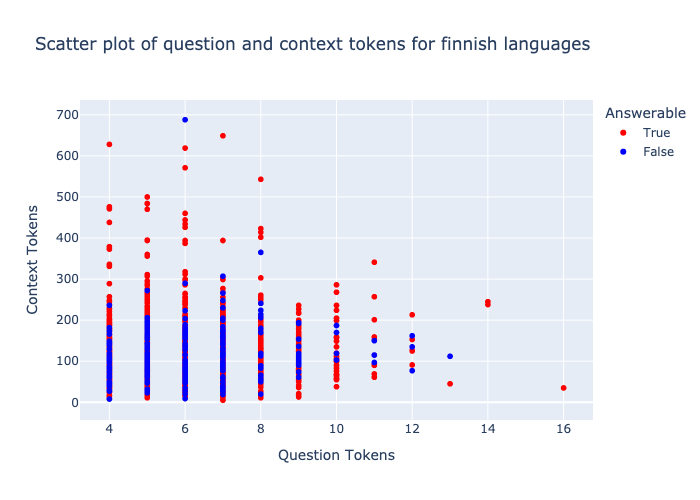
\includegraphics[width=0.25\textwidth]{week1_c_scatter_fi.png}
    \caption{Scatter plot for Finnish}
    \label{fig:scatter_week1_c_fi}
\end{figure}

\begin{figure}[ht]
    \centering
    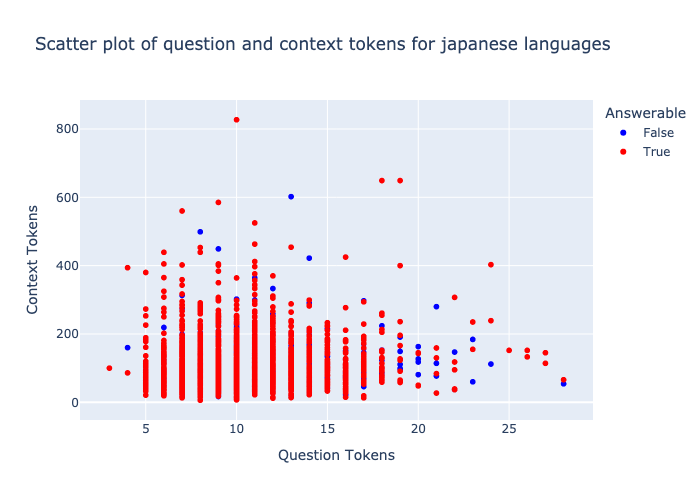
\includegraphics[width=0.25\textwidth]{week1_c_scatter_ja.png}
    \caption{Scatter plot for Japanese}
    \label{fig:scatter_week1_c_ja}
\end{figure}

\begin{figure}[ht]
    \centering
    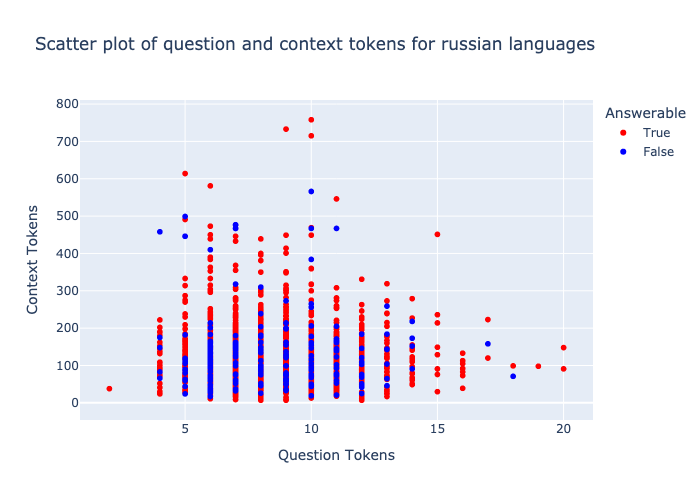
\includegraphics[width=0.25\textwidth]{week1_c_scatter_ru.png}
    \caption{Scatter plot for Russian}
    \label{fig:scatter_week1_c_ru}
\end{figure}

%% distillbert training logs

\begin{table}[ht]
    \centering
    \resizebox{0.9\columnwidth}{!}{
    \begin{tabular}{|c|c|c|c|}
        \hline
        Epoch & Language & Exact Match & F1 Score \\
        \hline
        0 & Fi & 16.10 & 17.27 \\
        0 & Ja & 19.96 & 16.49 \\
        0 & Ru & 12.88 & 17.24 \\
        \hline
        2 & Fi & 21.97 & 22.98 \\
        2 & Ja & 26.32 & 17.64 \\
        2 & Ru & 19.95 & 22.00 \\
        \hline
        4 & Fi & 27.27 & 27.39 \\
        4 & Ja & 21.27 & 19.28 \\
        4 & Ru & 18.94 & 21.50 \\
        \hline
        6 & Fi & 28.22 & 27.37 \\
        6 & Ja & 22.59 & 17.74 \\
        6 & Ru & 18.94 & 21.27 \\
        \hline
        8 & Fi & 27.27 & 26.68 \\
        8 & Ja & 23.25 & 18.49 \\
        8 & Ru & 18.43 & 22.26 \\
        \hline
        10 & Fi & 27.08 & 27.51 \\
        10 & Ja & 21.93 & 19.07 \\
        10 & Ru & 16.92 & 21.07 \\
        \hline
    \end{tabular}
    }
    \caption{Evaluation metrics for different languages at various epochs}
    \label{tab:evaluation_metrics}
\end{table}


\begin{figure}[ht]
    \centering
    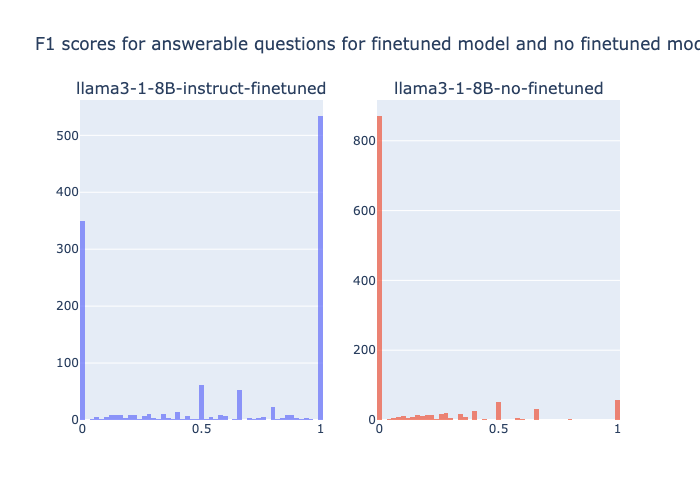
\includegraphics[width=0.5\textwidth]{week_41_f1_scores_answerable.png}
    \caption{F1 scores for answerable questions}
    \label{fig:week41_f1_scores_answerable}
\end{figure}




\subsection{References}

\nocite{Ando2005,andrew2007scalable,rasooli-tetrault-2015, rajpurkar-etal-2018-know, hu2021loralowrankadaptationlarge, risch2021semanticanswersimilarityevaluating}
\section{Bib\TeX{} Files}
\label{sec:bibtex}
\bibliography{custom}
\end{document}